\documentclass[10pt,a4paper, polish]{article}
\usepackage{lipsum}
\usepackage[normalem]{ulem}
\usepackage{array,multirow}
\usepackage[utf8]{inputenc}
\usepackage[T1]{fontenc}
\usepackage{amsfonts}
\usepackage{amssymb}
\usepackage{float}
\usepackage{graphicx}
\usepackage{latexsym,amsmath,amssymb,amsthm}
\usepackage{multicol}
\renewcommand{\arraystretch}{1,25}
\usepackage{breqn}
\usepackage{graphicx}
\usepackage{longtable} 
\usepackage{algorithm2e, algpseudocode}
\author{Jakub Jaśków}
\title{Obliczenia naukowe - Lista nr 3}

\begin{document}

\maketitle

\section{Metoda bisekcji}

\subsection*{Opis}
Napisanie funkcji znajdującej pierwiastki równania \textbf{metodą bisekcji}.
\subsection*{Rozwiązanie}
\subsubsection*{Opis algorytmu}
Metoda bisekcji stosowana jest do przybliżonego rozwiązywania równania $f(x) = 0$ w przedziale $[a,b]$. Funkcja $f(x)$ musi być określona i ciągła w tym przedziale oraz musi posiadać różne znaki na krańcach przedziału $[a,b]$, co gwarantuje istnienie przynajmniej jednego pierwiastka w tym przedziale. Rozwiązanie znajdowane jest za pomocą kolejnych przybliżeń. Z tego powodu należy określić dokładność, z którą chcemy otrzymać pierwiastek funkcji oraz dokładność wyznaczania samej funkcji.\\\\
W każdym przybliżeniu algorytm wyznacza środek $x_0$ przedziału $[a,b]$ jako średnią arytmetyczną krańców. Następnie sprawdzane jest, czy odległość tego środka od krańców przedziału jest mniejsza od założonej dokładności wyliczania pierwiastka. Jeśli tak, to algorytm kończy pracę z wynikiem w $x_0$. Jeśli nie, to wyznaczana jest wartość funkcji w punkcie $x_0$ i sprawdza się, czy odległość tej wartości od $0$ jest mniejsza od założonej dokładności wyznaczania funkcji. Jeśli tak, to algorytm kończy pracę z wynikiem w $x_0$.\\\\
W przeciwnym razie punkt $x_0$ dzieli przedział $[a,b]$ na dwie równe połowy: $[a,x_0]$ i $[x_0,b]$. Algorytm za nowy przedział $[a,b]$ przyjmuję tę połówkę, w której funkcja zmienia znak na krańcach i kontynuuje wyznaczanie pierwiastka funkcji.\\\\
Z opisu wynika, iż w każdym obiegu szerokość przedziału maleje dwukrotnie. Dzięki temu pierwiastek jest wyznaczany coraz bardziej dokładnie. Po dziesięciu obiegach szerokość przedziału maleje $210 = 1024$ razy.
\subsection*{Algorytm}
\begin{algorithm}[H]
\caption{Metoda bisekcji}
\label{alg:bis}
\DontPrintSemicolon
\SetKwFunction{proc}{mbisekcji}
\SetKwProg{myproc}{}{}{}
\myproc{\proc{f, a, b, delta, epsilon}}{
$u \leftarrow f(a)$\;
$v \leftarrow f(b)$\;
$e \leftarrow b - a$\;
$it \leftarrow 0$\;
\If {\texttt{sign}$(u) = $\texttt{sign}$(v)$}{
	\Return $err$ $1$\;
}
\While {$e > epsilon$}{
	$it \leftarrow it + 1$\;
	$e \leftarrow e / 2$\;
	$c \leftarrow a + e$\;
	$w \leftarrow f(c)$\;
	\If {$|e| < delta$ \textbf{or} $|w| < epsilon$}{
		\Return $c, w, it, 0$\;
	}
	\If {\texttt{sign}$(w) \neq $\texttt{sign}$(u)$}{
		$b \leftarrow c$\;
		$v \leftarrow w$\;
	}
	\Else {
		$a \leftarrow c$\;
		$u \leftarrow w$\;	
	}
}
}
\end{algorithm}

\begin{longtable}[l]{r  c  l}
%\begin{table}[!h]
%\centering
%\begin{tabular}{r  c  l}
\multicolumn{1}{l}{\textbf{Dane:}}&& \\
\texttt{f}&--&funkcja $f(x)$ zadana jako anonimowa funkcja (ang. anonymous function), \\
\texttt{a, b}&--&końce przedziału początkowego, \\
\texttt{delta, epsilon}&--&dokładności obliczeń, \\
&& \\
\multicolumn{1}{l}{\textbf{Wyniki:}}&& \\
\texttt{(r,v,it,err)}&--&czwórka, gdzie \\
\texttt{r}&--&przybliżenie pierwiastka równania $f(x) = 0$, \\
\texttt{v}&--&wartość $f(r)$, \\
\texttt{it}&--&liczba wykonanych iteracji, \\
\texttt{err}&--&sygnalizacja błędu \\
&&$0$ - brak błędu \\
&&$1$ - funkcja nie zmienia znaku w przedziale [a,b] \\
%\end{tabular}
\end{longtable}


\subsubsection*{Notatki}
1. Punkt środkowy $c$ obliczamy poprzez $c \leftarrow a + (b - a)/2$. Instrukcja $c \leftarrow (a + b)/2$ mogłaby spowodować, że w ekstremalnych przypadkach $c \notin [a, b]$.\\\\
2. Pozbywamy się mnożenia przy $f(a)f(c) < 0$, następstwem którego mógł by być nadmiar lub niedomiar, instrukcją $sign(w) \neq sign(u)$.\\\\
3. Uwzględniamy trzy możliwości zakończenia algorytmu:\\
\quad $e > epsilon$ mówi kiedy jest możliwa iteracja w danym przedziale.\\
\quad Błąd jest dostatecznie mały ($abs(e) < delta$).\\
\quad $f(c)$ jest dostatecznie bliskie zeru ($abs(w) < epsilon$).

\section{Metoda Newtona}

\subsection*{Opis problemu}
Napisanie funkcji znajdującej pierwiastki równania \textbf{metodą Newtona}.
\subsection*{Rozwiązanie}
\subsubsection*{Opis algorytmu}
Metoda \textbf{Newtona} (stycznych) wyszukująca pierwiastki funkcji opiera się na \emph{linearyzacji funkcji}, czyli zastąpieniu $f(x)$ funkcją liniową, będącą sumą dwóch początkowych składników we wzorze Taylora dla $f$. Zbieżność metody stycznych jest kwadratowa, co czyni ją (średnio)szybszą od metod \textbf{bisekcji} czy siecznych. Gdy przybliżenia otrzymane za pomocą metody \textbf{Newtona} stają się bliskie pierwiastka, staje się ona na tyle szybko zbieżna, że kilka przybliżeń pozwala osiągnąć maksymalną dokładność. Metoda stycznych nie zawsze jest zbieżna, więc na ogół stosuje się ją w razem z innymi metodami zbieżnymi globalnie. Kłopotliwa jest także konieczność obliczenia pochodnej, co może sprawiać problemy dla niektórych funkcji.
\subsubsection*{Algorytm}
\begin{algorithm}[H]
\caption{Metoda Newtona}
\label{alg:new}
\DontPrintSemicolon
\SetKwFunction{proc}{mstycznych}
\SetKwProg{myproc}{}{}{}
\myproc{\proc{f, $p_f$, $x_0$, delta, epsilon, maxit}}{
$v \leftarrow f(x_0)$\;

\If {$|v| < epsilon$}{
	\Return $x_0, v, 0, 0$\;
}

\If {$|p_f(x_0)| < epsilon$}{
	\Return $err$ $2$\;
}

\For {$it \leftarrow 1$ \KwTo $maxit$}{
	$x_1 \leftarrow x_0 - (v/p_f(x_0))$\;
	$v \leftarrow f(x_1)$\;
	\If {$|x_1 - x_0| < delta$ \textbf{or} $|v| < epsilon$}{
		\Return $x_1, v, it, 0$\;
	}
	$x_0 \leftarrow x_1$\;
}
\Return $err$ $1$\;
}
\end{algorithm} 
\begin{longtable}[l]{r  c  l}
\multicolumn{1}{l}{\textbf{Dane:}}&& \\
\texttt{f, pf}&--&funkcja $f(x)$ oraz pochodna $f'(x)$ zadane jako anonimowe funkcje, \\
\texttt{x0}&--&przybliżenie początkowe, \\
\texttt{delta, epsilon}&--&dokładności obliczeń, \\
\texttt{maxit}&--&maksymalna dopuszczalna liczba iteracji, \\
&& \\
\multicolumn{1}{l}{\textbf{Wyniki:}}&& \\
\texttt{(r,v,it,err)}&--&czwórka, gdzie \\
\texttt{r}&--&przybliżenie pierwiastka równania $f(x) = 0$, \\
\texttt{v}&--&wartość $f(r)$, \\
\texttt{it}&--&liczba wykonanych iteracji, \\
\texttt{err}&--&sygnalizacja błędu \\
&&$0$ - metoda zbieżna \\
&&$1$ - nie osiągnięto wymaganej dokładności w \texttt{maxit} iteracji \\
&&$2$ - pochodna bliska zeru \\
\end{longtable}

\subsubsection*{Notatki}
Na początku algorytmu sprawdzamy: \\
1. Wartość funkcji dla przybliżenia początkowego jest wystarczająco bliska zeru - zwracany jest wynik.\\
2. Pochodna jest bliska zeru - niemożliwe jest wtedy zastosowanie metody.\\\\ Następnie wyznaczane są kolejne przybliżenia zera funkcji, które są dane rekurencyjnym wzorem $$x_{n+1} := x_n - \dfrac{f(x_n)}{f'(x_n)}$$. Algorytm kończy się kiedy znaleziony pierwiastek mieści się w dokładności, lub odległości pomiędzy przybliżeniami są wystarczająco niewielkie. Błąd zwracamy jeżeli żadne z powyższych warunków nie zostanie spełniony.

\section{Metoda siecznych}

\subsection*{Opis}
Napisanie funkcji wyznaczającej pierwiastki równania $f(x) = 0$ metodą \textbf{siecznych}.
\subsection*{Rozwiązanie}
\subsubsection*{Opis algorytmu}
Metoda \textbf{siecznych} powstała na skutek próby eliminacji obliczania pochodnej dla metody Newtona. Aby tego dokonać $f'(x)$ zastąpiono ilorazem różnicowym: $$f'(x) \approx \dfrac{f(x_n)-f(x_{n-1})}{x_n-x_{n-1}}$$.\\\\ Równość ta, wynikająca z definicji pochodnej, skutkuje właśnie metodą siecznych $$x_{n+1} := x_n - f(x_n)\dfrac{x_n-x_{n-1}}{f(x_n)-f(x_{n-1})}$$\\\\
$x_{n+1} = x_n + x_{n-1}$ więc potrzebujemy $n_0$ oraz $n_1$, jednak każde nowe $x_{n+1}$ wymaga jednej wartości funkcji $f$. Metoda \textbf{siecznych} zbiega wolniej niż metoda Newtona, natomiast każdy jej krok wymaga obliczenia tylko \textbf{jednej} wartości funkcji, zamiast dwóch - $f(x)$ i $f'(x)$.
\subsubsection*{Algorytm}
\begin{algorithm}[H]
\caption{Metoda siecznych}
\label{alg:sie}
\DontPrintSemicolon
\SetKwFunction{proc}{msiecznych}
\SetKwProg{myproc}{}{}{}
\myproc{\proc{f, $x_0$, $x_1$, delta, epsilon, maxit}}{
$f_{x_0} \leftarrow f(x_0)$\;
$f_{x_1} \leftarrow f(x_1)$\;

\For {$it \leftarrow 1$ \KwTo $maxit$}{
	\If {$|f_{x_0}| > |f_{x_1}|$}{
		$x_0 \leftrightarrow x_1$\;
		$f_{x_0} \leftrightarrow f_{x_1}$\;
	}
	$s \leftarrow (x_1 - x_0)/(f_{x_1} - f_{x_0})$\;
	$x_1 \leftarrow x_0$\;
	$f_{x_1} \leftarrow f_{x_0}$\;
	$x_0 \leftarrow x_0 - (f_{x_0} \times s)$\;
	$f_{x_0} \leftarrow f(x_0)$\;
	\If {$|x_1 - x_0| < delta$ \textbf{or} $|f_{x_0}| < epsilon$}{
		\Return $x_0, f_{x_0}, it, 0$\;
	}
}
\Return $err$ $1$\;
}
\end{algorithm}
\begin{longtable}[l]{r  c  l}
%\begin{table}[!h]
%\centering
%\begin{tabular}{r  c  l}
\multicolumn{1}{l}{\textbf{Dane:}}&& \\
\texttt{f}&--&funkcja $f(x)$ zadana jako anonimowa funkcja, \\
\texttt{x0, x1}&--&przybliżenia początkowe, \\
\texttt{delta, epsilon}&--&dokładności obliczeń, \\
\texttt{maxit}&--&maksymalna dopuszczalna liczba iteracji, \\
&& \\
\multicolumn{1}{l}{\textbf{Wyniki:}}&& \\
\texttt{(r,v,it,err)}&--&czwórka, gdzie \\
\texttt{r}&--&przybliżenie pierwiastka równania $f(x) = 0$, \\
\texttt{v}&--&wartość $f(r)$, \\
\texttt{it}&--&liczba wykonanych iteracji, \\
\texttt{err}&--&sygnalizacja błędu \\
&&$0$ - metoda zbieżna \\
&&$1$ - nie osiągnięto wymaganej dokładności w \texttt{maxit} iteracji \\
%\end{tabular}
\end{longtable}

Algorytm metody przedstawionej powyżej przestawia wartości $x_0$ i $x_1$, kiedy wymaga tego utrzymanie nierówności $|f_{x_0}| \leq |f_{x_1}|$. Algorytm kończy się kiedy znaleziony pierwiastek mieści się w dokładności, lub odległości pomiędzy przybliżeniami są wystarczająco niewielkie. Błąd zwracamy jeżeli żadne z powyższych warunków nie zostanie spełniony.
\section{zad}

\subsection*{Opis}
Wyznaczanie pierwiastka równania $\sin{x} = -(\frac{1}{2}x)^2$ z użyciem metod:\\
1. bisekcji (na przedziale początkowym $[1.5, 2.0]$,\\
2. Newtona (dla przybliżenia początkowego $x_0 = 1.5$,\\  
3. siecznych (dla przybliżeń początkowych $x_0 = 1.0, x_1 = 2.0$.\\\\
Gdzie $\delta = \frac{1}{2}10^{-5}$, $\epsilon = \frac{1}{2}10^{-5}$.

\subsection*{Rozwiązanie}
Podstawienie funkcji $f(x) = \sin{x}-(\frac{1}{2}x)^2$, jej pochodnej $f'(x) = \cos{x} - \frac{1}{2}x$ do metod zaimplementowanych w zadaniach 1-3. $maxIt = 32$.

\subsection*{Wyniki}

\begin{table}[h]
        \centering
        \footnotesize
\begin{tabular}{c|c|c|c|c}
Metoda    & {Miejsce zerowe ($x_0$)} 	& {Wartość funkcji ($f(x_0)$)} 	& Liczba iteracji	& Błąd \\ \hline
Bisekcji  & 1.9337539672851562       	&-2.7027680138402843e-7			& 16 				& 0 \\ 
Newtona   &  1.933753779789742			&-2.2423316314856834e-8			& 4 				& 0 \\ 
Siecznych & 1.9337539405015145			&-2.3487103129049558e-7			& 5 				& 0 \\ 
\end{tabular}
\caption{Pierwiastki równania $f(x) = \sin{x}-(\frac{1}{2}x)^2$ obliczone przy pomocy implementacji metod z zadań 1-3.}
\label{table:1}
\end{table}	

\subsection*{Wnioski}
Na tabeli powyżej bardzo dobrze widać różnicę w liczbie iteracji potrzebnych do wyznaczenia pierwiastków równania. Wartości te zgadzają się z naszymi przewidywaniami, bowiem metoda bisekcji posiada zbieżność liniową, metoda Newtona kwadratową natomiast metoda siecznych ok $\approx 1.62$ (nadliniowo). Metoda bisekcji nie jest, jak mogło by się zdawać, najwolniejsza, ale "najstabilniejsza". Znalazła ona wartość najbliższą zeru, oraz jest stabilna globalnie. Dla danych podanych w zadaniu metoda Newtona oraz metoda siecznych zbiegają szybciej niż metoda bisekcji, lecz dla innej funkcji lub innych przedziałów obserwacje te mogą się różnić.

\section{zad}

\subsection*{Opis}
Przy użyciu metody bisekcji znajdź wartość $x$, dla której przecinają się wykresy funkcji $y=3x$ oraz $y=e^x$.

\subsection*{Rozwiązanie}
Znalezienia miejsc zerowych funkcji $f(x) = e^x - 3x$ przy użyciu metody bisekcji stworzonej w zadaniu pierwszym.\\
Dokładności:\\
$\delta = 10^{-4}$\\
$\epsilon = 10^{-4}$\\
Wybrane przedziały: $[0, 1]$, $[1, 2]$.

\subsection*{Wyniki}
Punkty przecięcia:\\
$0.619140625$ dla przedziału $[0,1]$,\\
$1.5120849609375$ dla przedziału $[1,2]$.

\begin{table}[h]
        \centering
        \footnotesize
\begin{tabular}{c|c|c}
& $x_0$ & $x_1$ \\ \hline
Przedział & $[0, 1]$ & $[1, 2]$ \\ 
Wartość & $0.619140625$ & $1.5120849609375$ \\ 
Niedokładność $|f(x_i)|$ & $9.066320343276146 \times 10^{-5}$ & $7.618578602741621 \times 10^{-5}$ \\
Liczba iteracji &$9$&$13$ \\
\end{tabular}
\caption{Miejsca zerowe funkcji $f(x) = e^x - 3x$ obliczone za pomocą metody bisekcji.}
\label{table:2}
\end{table}	

\subsection*{Wnioski}
Wiedza z analizy matematycznej jest niezbędna przy doborze parametrów początkowych do poszczególnych metod szukania pierwiastków równania. Jeśli spełnimy wszystkie jej założenia, metoda bisekcji gwarantuje nam znalezienie "jakiegoś" pierwiastka równania. Jeżeli natomiast zależy nam na znalezieniu wszystkich rozwiązań, musimy skorzystać z naszej wiedzy na temat analizy matematycznej. Analiza samego problemu pomoże nam dobrać odpowiedni przedział początkowy, co pozwoli na znaczne przyśpieszenie obliczeń w przypadku zastosowania metody stycznych czy metody siecznych.
\section{zad}
\subsection*{Opis}
Znajdź pierwiastki funkcji $f_1(x)=e^{1-x}-1$ i $f_2(x)=xe^{-x}$ przy pomocy metod bisekcji, stycznych oraz siecznych z dokładnością: $\delta=10^{-5}$, $\epsilon=10^{-5}$.

\subsection*{Rozwiązanie}
Zaimplementuj wymienione wyżej funkcje (przy użyciu metod z zadań 1-3) oraz oblicz ich pochodne. Przeprowadzona została analiza funkcji $f_1$ i $f_2$, które zostały przedstawione na wykresie \ref{fig:zad61}, na podstawie której dobrano parametry początkowe.

\begin{figure}[H]
\centering
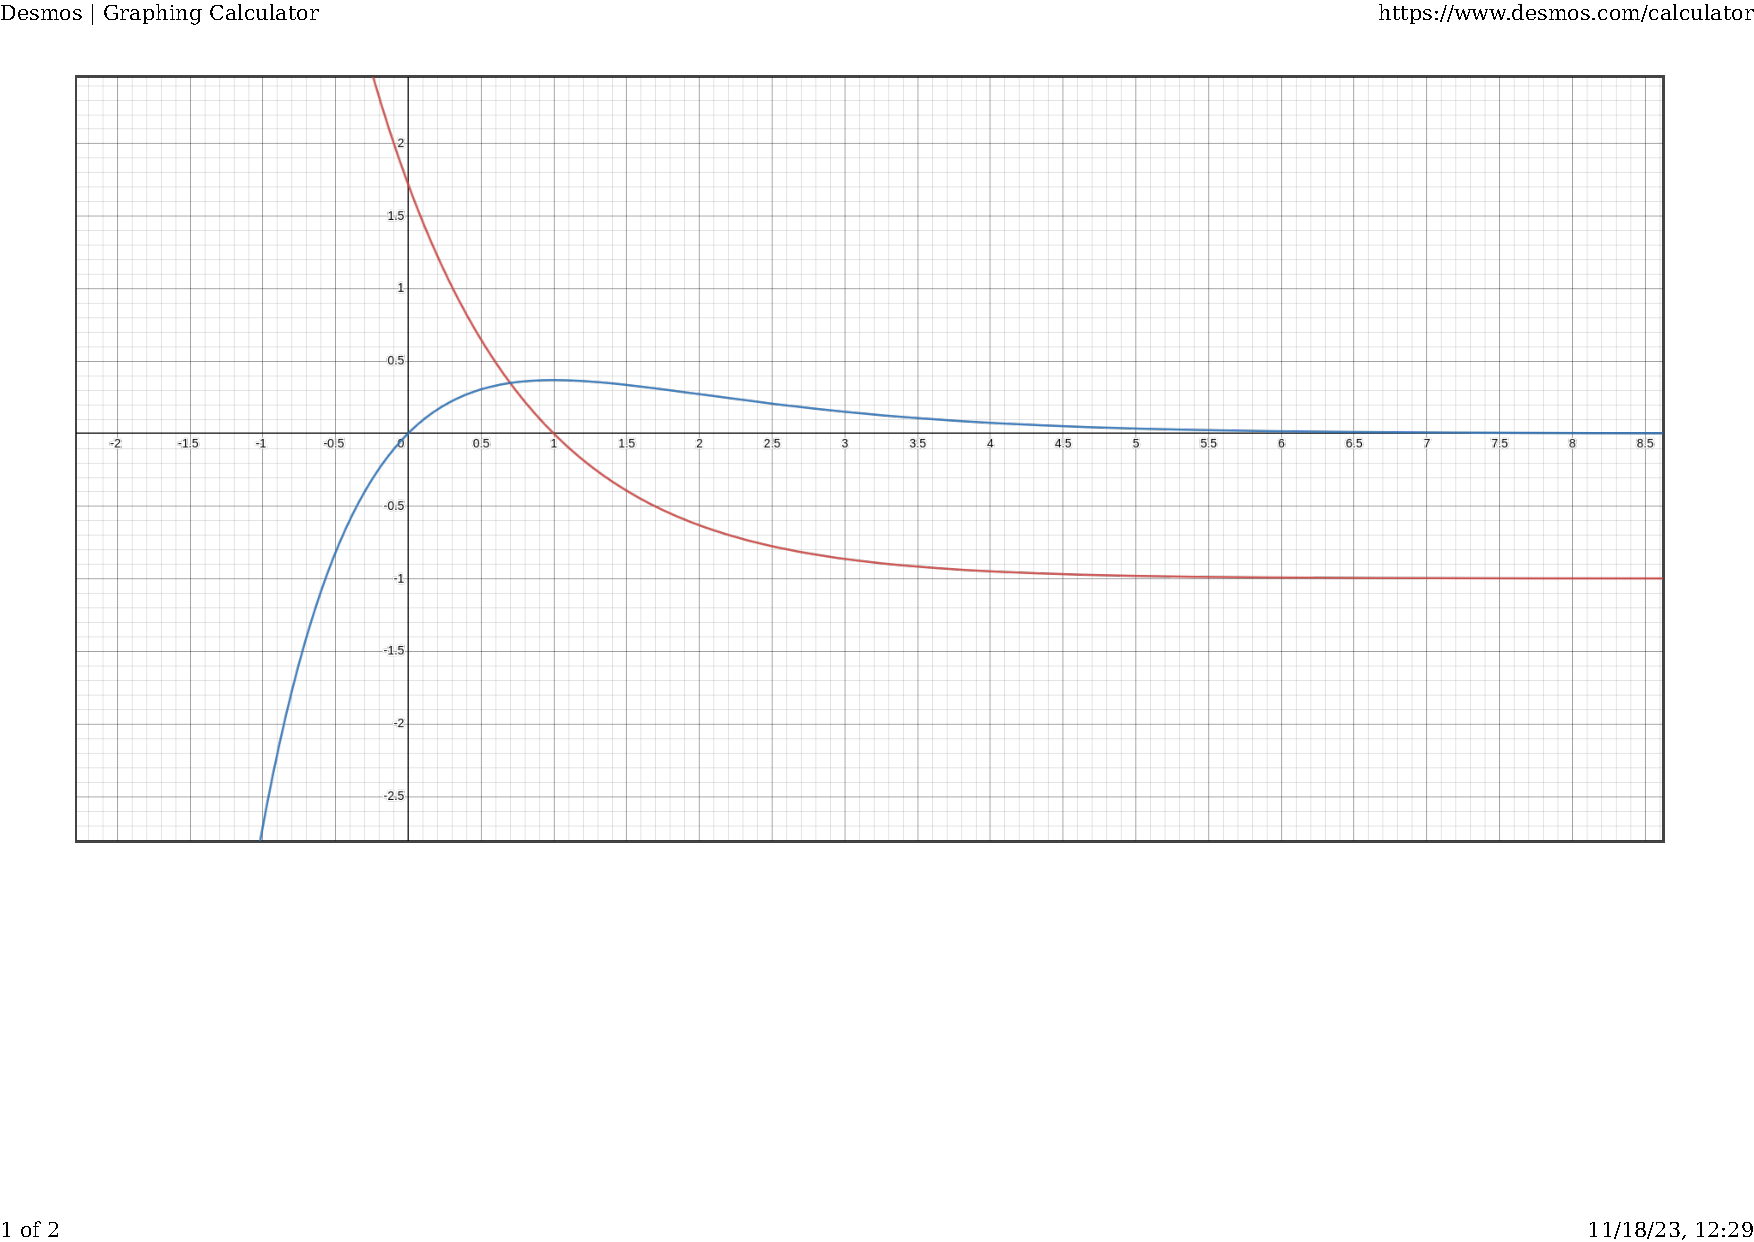
\includegraphics[width=1\textwidth]{zad6_1}\hfill
\caption{Wykresy funkcji $f(x)=e^{1-x}-1$ oraz $g(x)=xe^{-x}$ wykonane w kalkulatorze graficznym Desmos} \label{fig:zad61}
\end{figure} 

\subsection*{Wyniki}
Łatwo zauważyć, że poprawnymi rozwiązaniami dla $f_1$ i $f_2$ jest odpowiednio $-1$ i $0$.

\begin{table}[H]
        \centering
        \footnotesize
\begin{tabular}{c|c|c|c}
Przedział& {$r$} & {$f(r)$} & Liczba iteracji \\ \hline
\multicolumn{4}{c}{$f_1$} \\ \hline
$[0.0,1.5]$&1.0000076293945312&-7.6293654275305656e-6&16 \\
$[0.5,3.0]$&0.9999923706054688&7.629423635080457e-6&16 \\
$[-4.0,4.0]$&1.0&0.0&3 \\
$[0.0,100.0]$&0.9999990463256836&9.536747711536009e-7&22 \\
$[-10.0,2000.0]$&1.0000018030405045&-1.803038878978036e-6&27 \\ \hline
\multicolumn{4}{c}{$f_2$} \\ \hline
$[-0.5,1.0]$&-7.62939453125e-6&-7.629452739132958e-6&16 \\
$[-0.25,1.5]$&-7.62939453125e-6&-7.629452739132958e-6&15 \\
$[-1.0,6.0]$&-3.814697265625e-6&-3.814711817567984e-6&18 \\
$[-1.5,100.0]$&49.25&2.010958004139294e-20&1 \\
$[-5.0,1000.0]$&497.5&4.318056675122884e-214&1 \\
\end{tabular}
\caption{Miejsca zerowe $f_1$ i $f_2$ obliczone za pomocą metody bisekcji.}
\label{table:3}
\end{table}

\begin{table}[H]
        \centering
        \footnotesize
\begin{tabular}{c|c|c|c|c}
$x_0$& {$r$} & {$f(r)$} & Liczba iteracji & Błąd \\ \hline
\multicolumn{5}{c}{$f_1$} \\ \hline
-1.0&0.9999922654776594&7.734552252003368e-6&5&0 \\
0.0&0.9999984358892101&1.5641120130194253e-6&4&0 \\
1.0&1.0&0.0&0&0 \\
2.0&0.9999999810061002&1.8993900008368314e-8&5&0 \\
5.0&0.9999996427095682&3.572904956339329e-7&54&0 \\
7.0&0.9999999484165362&5.15834650549607e-8&401&0 \\
8.0&{---}&{---}&{---}&1 \\
13.0&{---}&{---}&{---}&2 \\ \hline
\multicolumn{5}{c}{$f_2$} \\ \hline
-2.0&-1.425500682806244e-9&-1.425500684838296e-9&7&0 \\
-1.0&-3.0642493416461764e-7&-3.0642502806087233e-7&5&0 \\
0.0&0.0&0.0&0&0 \\
0.5&-3.0642493416461764e-7&-3.0642502806087233e-7&5&0 \\
1.0&{---}&{---}&{---}&2 \\
2.0&14.398662765680003&8.036415344217211e-6&10&0 \\
5.0&15.19428398343915&3.827247505782987e-6&9&0 \\
100.0&100.0&3.7200759760208363e-42&0&0 \\

\end{tabular}
\caption{Miejsca zerowe $f_1$ i $f_2$ obliczone za pomocą metody stycznych.}
\label{table:4}
\end{table}

\begin{table}[H]
        \centering
        \footnotesize
\begin{tabular}{c|c|c|c|c|c}
$x_0$&$x_1$& {$r$} & {$f(r)$} & Liczba iteracji & Błąd \\ \hline
\multicolumn{5}{c}{$f_1$} \\ \hline
-1.0&2.0&1.0000009310146594&-9.310142259355558e-7&7&0 \\
0.5&3.0&0.9999998801054126&1.1989459447470097e-7&6&0 \\
-3.0&4.0&0.9999924734799833&7.526548341019179e-6&1500&0 \\
-2.0&6.0&5.229263398675002&-0.9854368861925255&5&0 \\
10.0&100.0&{---}&{---}&{---}&1 \\ \hline
\multicolumn{5}{c}{$f_2$} \\ \hline
-1.0&0.5&3.201418966654486e-7&3.2014179417463104e-7&7&0 \\
-0.25&1.5&5.662892187393383e-7&5.662888980559498e-7&7&0 \\
2.0&6.0&14.386737398698989&8.12609044213971e-6&12&0 \\
10.0&20.0&20.00090808104888&4.118752554492817e-8&1&0 \\
-2.0&100.0&100.0&3.7200759760208363e-42&1&0 \\

\end{tabular}
\caption{Miejsca zerowe $f_1$ i $f_2$ obliczone za pomocą metody siecznych.}
\label{table:5}
\end{table}

\subsection*{Wnioski}

Po przeanalizowaniu wyników z tabeli 6 możemy stwierdzić, że metoda \textbf{bisekcji}:\\
1. \textbf{$f_1$} - metoda ta zbiega do zera nawet dla bardzo dużych przedziałów, jeżeli przyjmiemy wystarczającą liczbę iteracji.\\
2. \textbf{$f_2$} - należy uważać na dobór przedziałów nawet stosując metodę bisekcji, ponieważ $f_1$ osiąga zero w nieskończoności. Przyjęcie dużego przedziału początkowego skutkować może zakończeniem obliczeń po jednej iteracji, gdyż wartość będzie dostatecznie bliska wartości zera, natomiast odległa od rzeczywistego pierwiastka $f_2$. \\\\

Po przeanalizowaniu wyników z tabeli 7 możemy stwierdzić, że metoda \textbf{Newtona}:\\
1. \textbf{$f_1$} - dla wartości oddalonych od zera liczba iteracji rośnie, co skutkuje rozbieżnością metody dla dużej liczb iteracji. Od pewnego momentu funkcja $f_1$, bardzo wolno maleje, więc jej pochodna osiąga wartość bliską zeru, co czyni zastosowanie metody Newtona niemożliwym.\\
2. \textbf{$f_2$} - pochodna zeruje się dla $x_0 = 1$. Dla wszystkich wartości przybliżenia początkowego, które są większe od jedynki, metoda nie zbiega do faktycznego zera funkcji, ale znajduje wartość dostatecznie bliską zeru. Dzieje się tak, bowiem $lim_{x \to \infty}f_2(x) = 0$. \\\\

Po przeanalizowaniu wyników z tabeli 8 możemy stwierdzić, że metoda \textbf{siecznych}:\\
1. \textbf{$f_1$} - dla przybliżeń początkowych oddalonych od zera możemy obserwować rozbieżność(jak w metodzie \textbf{Newtona}).\\ Ciekawym wynikiem jest wartość uzyskana dla $x_0 = -2$ i $x_1 = 6$. Metoda nie znajduje wartości funkcji bliskiej zeru, ale w pewnym momencie warunek $|x_1 - x_0| < delta$ staje się prawdą, kończąc działanie algorytmu. Dzieje się tak, ponieważ różnica między wartościami funkcji $f_1$ w $x_0 = -2$ i $x_1 = 6$ jest bardzo duża i kolejne przybliżenie wyznaczane jest bardzo blisko $x_1$.\\
2. \textbf{$f_2$} - analogicznie do metody \textbf{Newtona}.

\end{document}
